\documentclass[11pt]{article}
\usepackage[letterpaper,landscape,margin=0.55in]{geometry}
\usepackage{graphicx,booktabs,amsmath,array,fancyhdr,xcolor}
\usepackage[T1]{fontenc}
\usepackage{lmodern}
\setlength{\parindent}{0pt}
\setlength{\parskip}{5pt}
\pagestyle{fancy}\fancyhf{}\fancyfoot[C]{\thepage}
\renewcommand{\headrulewidth}{0pt}
\newcommand{\titleline}[1]{{\Large\bfseries #1}\par\vspace{3pt}}
\begin{document}
\titleline{Theory benchmark: optimized prices}
\small
Normal gamma: mean 0, SD 1.25; $\beta=2$, $\alpha=-1$, zero marginal cost, $\delta=1$.
Uniform observes history but not gamma; Informed observes its quintile. Neither learns.
All offered prices are constrained to be nonnegative.
\begin{center}
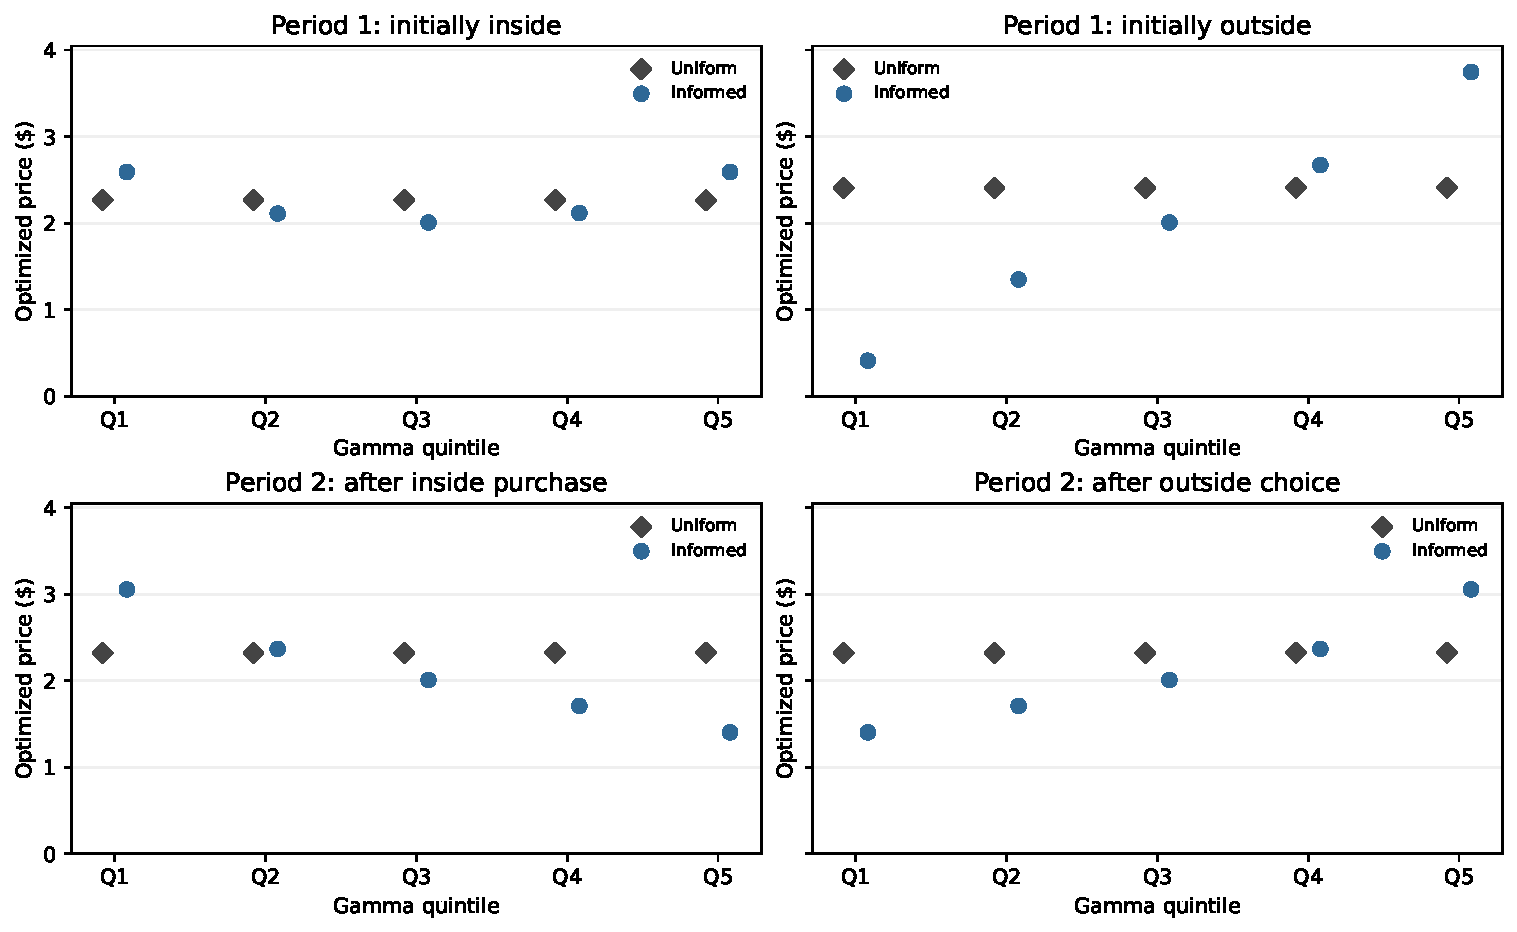
\includegraphics[width=9.5in,height=5.4in,keepaspectratio]{advisor_assets/theory_prices.pdf}
\end{center}
Each quintile has 20\% probability. Points are optimized offers at the indicated decision,
without averaging over future purchase histories. The informed firm knows the quintile, not exact gamma.
\newpage
\titleline{Theory benchmark: welfare and revenue}
\small
Percentage changes are Informed minus Uniform, divided by the absolute Uniform baseline.
CS is consumer surplus; TW is total welfare.
\begin{center}
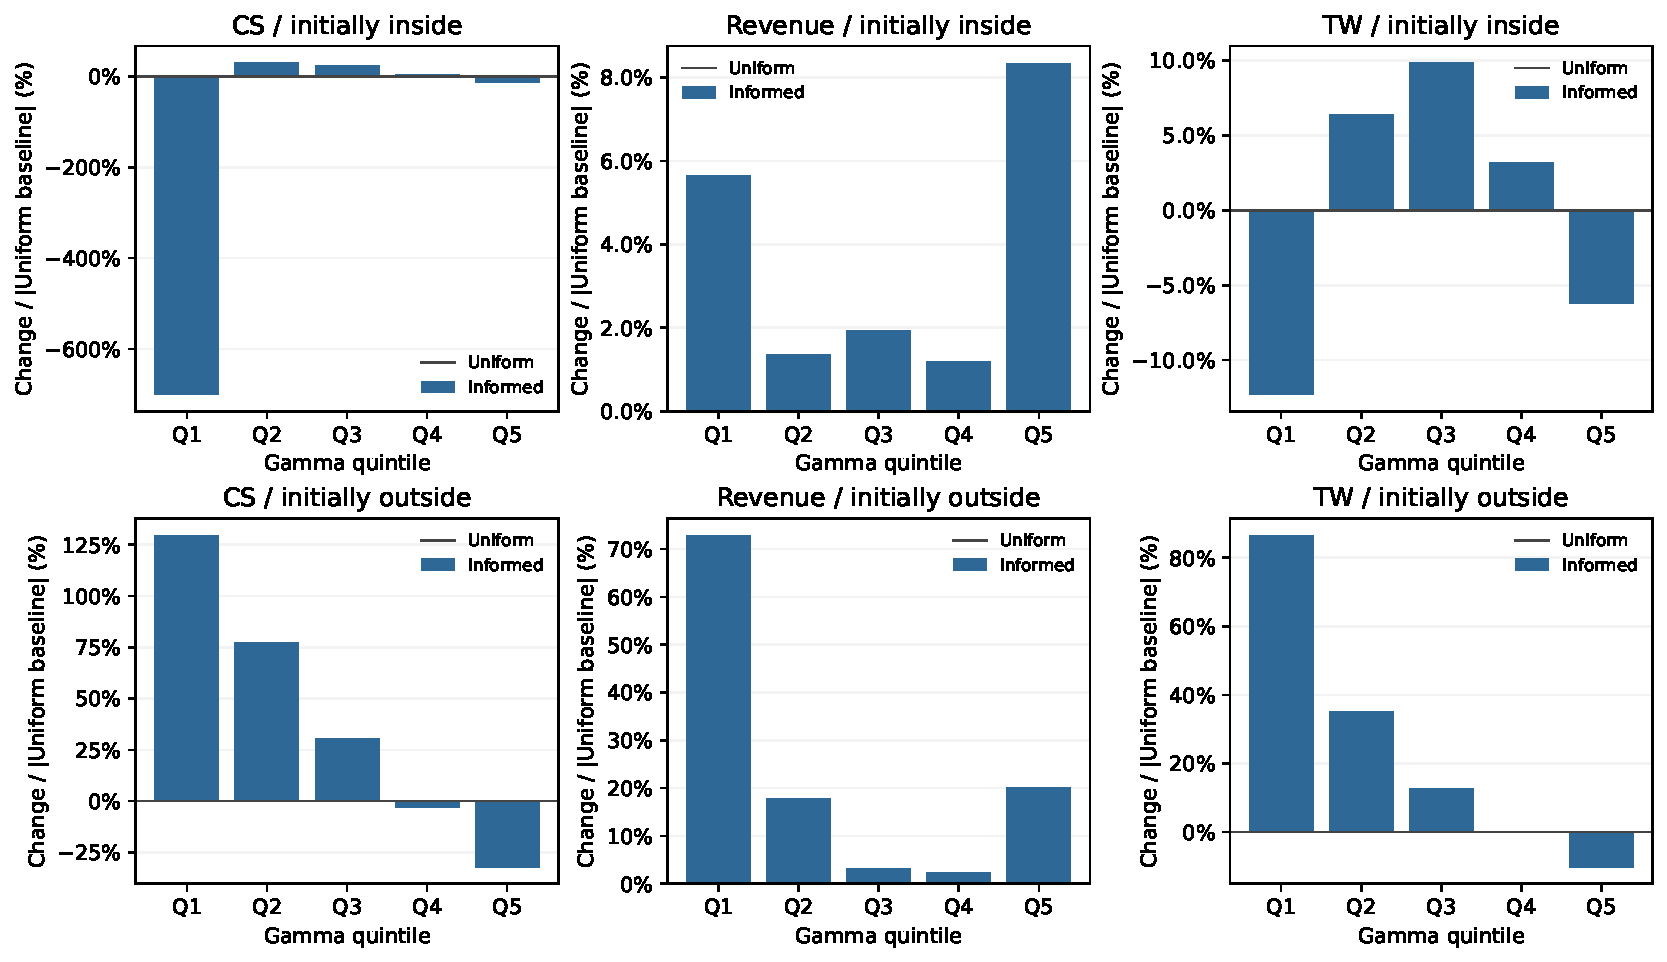
\includegraphics[width=9.8in,height=5.95in,keepaspectratio]{advisor_assets/theory_welfare.pdf}
\end{center}
\newpage
\titleline{Plain prices: trimmed, flavor switching specification}
\small
Gamma is trimmed at the 5th and 95th percentiles, with the retained distribution renormalized.
All offered prices are constrained to be nonnegative.
\begin{center}
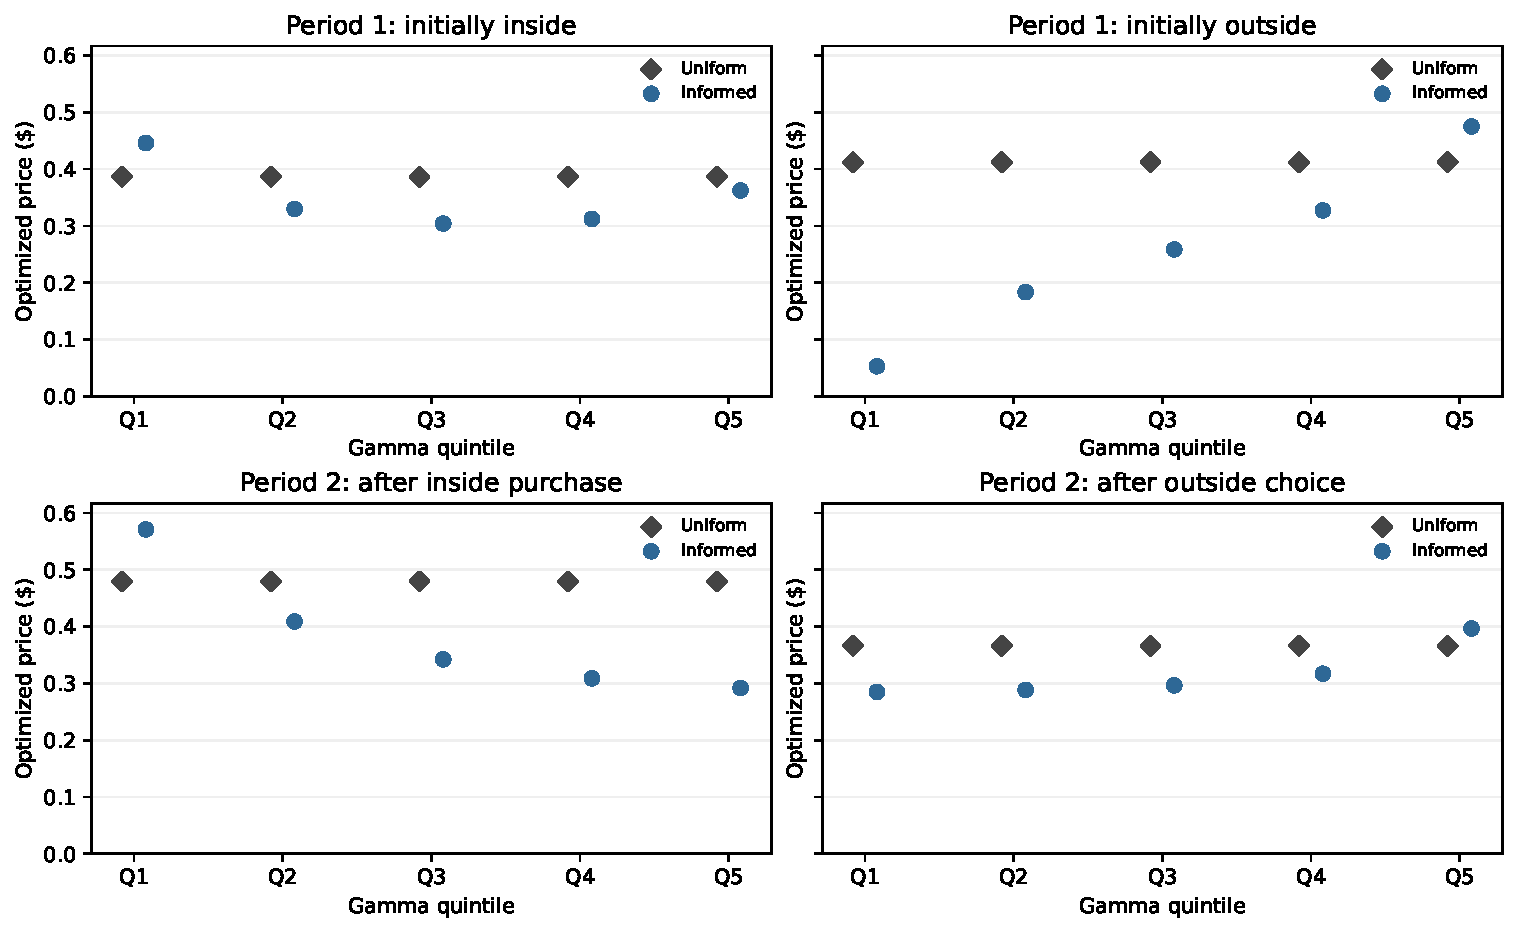
\includegraphics[width=9.5in,height=5.35in,keepaspectratio]{advisor_assets/plain_prices.pdf}
\end{center}
Inside means plain yogurt; outside means no plain yogurt (berry, other yogurt, or no yogurt).
Q1--Q5 each contain 20\% of the retained distribution (18\% of original mass).
\newpage
\titleline{Plain welfare: trimmed, flavor switching specification}
\small
Percentage changes are Informed minus Uniform, divided by the absolute Uniform baseline.
CS is consumer surplus; TW is total welfare.
\begin{center}
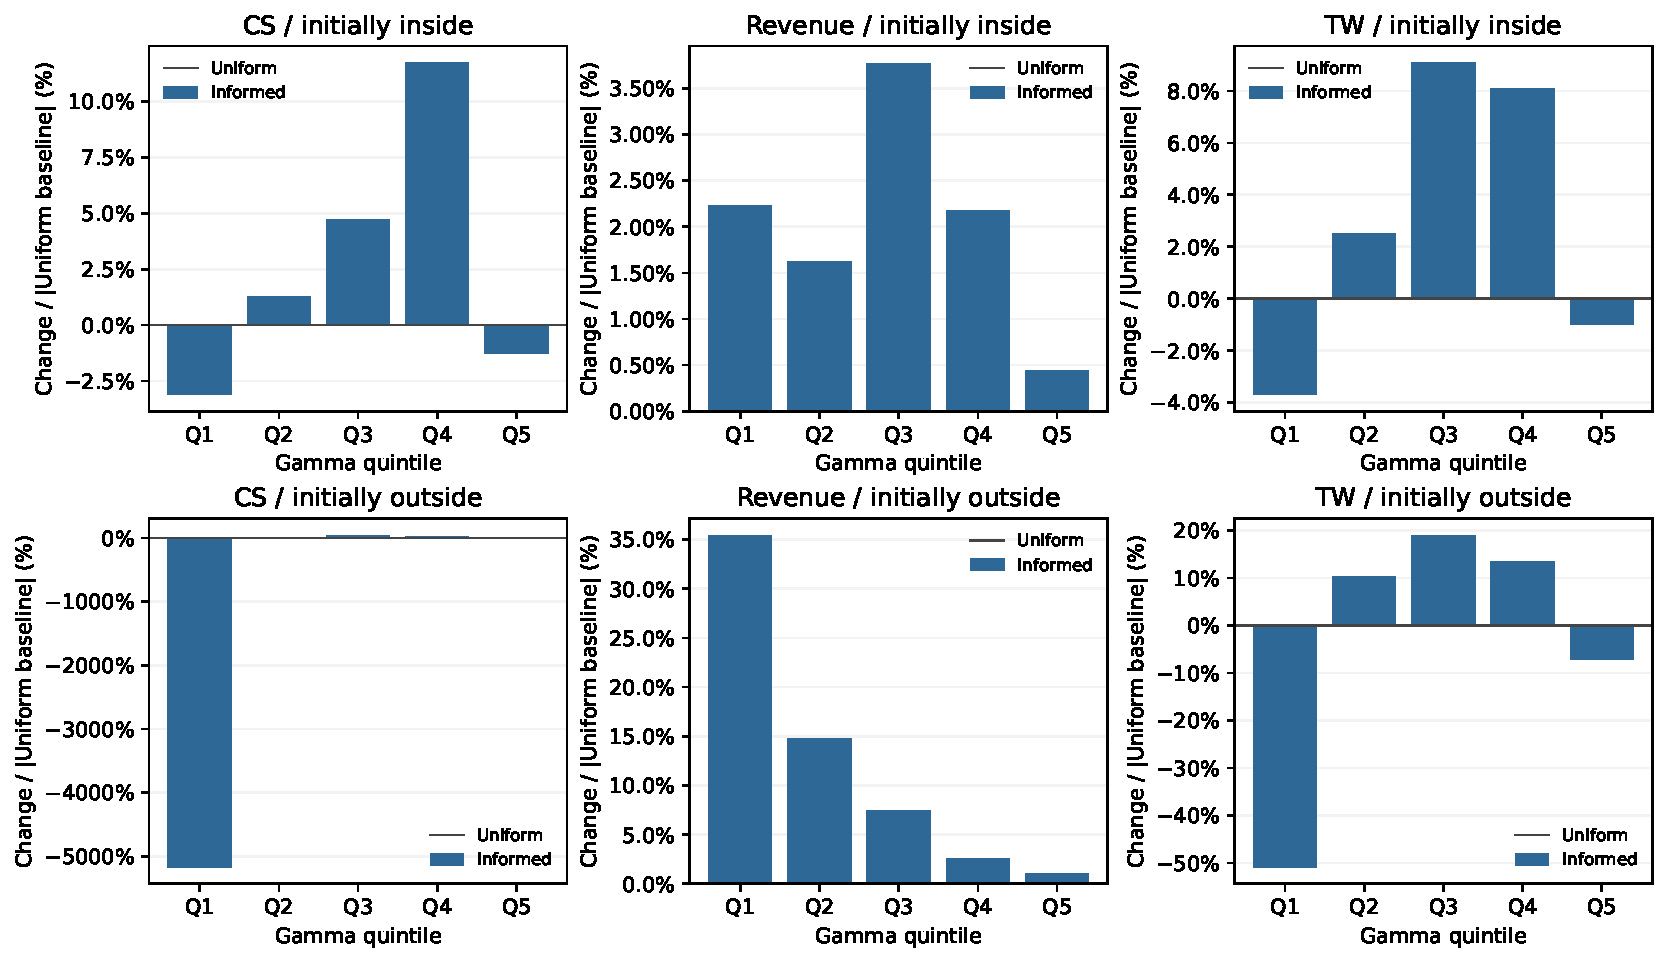
\includegraphics[width=9.8in,height=5.95in,keepaspectratio]{advisor_assets/plain_welfare.pdf}
\end{center}
\newpage
\titleline{Welfare outliers: dollar levels and percentage changes}
\small
Trimmed, flavor switching specification. Values are expected dollars per consumer
over the two modeled shopping weeks, conditional on the stated initial state and quintile.
CS is consumer surplus; TW is total welfare (CS plus revenue at zero cost).
\vspace{10pt}
\begin{center}
\renewcommand{\arraystretch}{1.4}
\begin{tabular}{lllrrrr}
\toprule
Initial state & Quintile & Metric & Uniform (\$) & Informed (\$) & Change (\$) & Change (\%)\\
\midrule
Outside & Q1 & CS & -0.00005 & -0.00285 & -0.00280 & -5,172.9\% \\
Outside & Q1 & TW & 0.00322 & 0.00158 & -0.00164 & -50.9\% \\
\addlinespace
Inside & Q1 & CS & -1.02946 & -1.06151 & -0.03205 & -3.1\% \\
Inside & Q1 & TW & -0.61998 & -0.64290 & -0.02293 & -3.7\% \\
\addlinespace
Outside & Q5 & CS & 0.25978 & 0.22732 & -0.03246 & -12.5\% \\
Outside & Q5 & TW & 0.42930 & 0.39869 & -0.03061 & -7.1\% \\
\bottomrule
\end{tabular}
\end{center}
\end{document}
